\chapter{Literature review}
\label{LR}

\section{Methods of Modelling Phages and Bacteria}
There are numerous ways to model the interactions between phages and bacteria.
Models can be built at a molecular level, where the model simulates the mechanical and chemical behavior of a phage as it interacts with the surface of a bacterium using computational chemistry methods.
On the other end of the spectrum, a different type of model can be built where populations of phages, bacteria, and resources can be modeled using Ordinary Differential Equations (ODEs) or Delay Differential Equations (DDEs).
DDEs are similar to ODEs, except where when ODEs are calculating the values of the equations at time $t$ using time $t-1$, DDEs can, but don't have to, use the value of the equation at time $t-\tau$, where $1 \leq \tau \leq t$. 
DDEs are a generalized version of ODEs and are significantly harder to analyze and find stability conditions than ODEs due to the dependence on the past \cite{liExploringComplicatedBehaviors2023}. \newline
One way to introduce DDE like behavior is to force agents to go through stages, causing a delay in other events. 
For example, in the paper \citet{gengUsingBacterialPopulation2024}, infected bacteria go through $M$ stages of infection, before lysing. 
The more stages there are, the longer the delay in seeing a rise in phage population. By changing the value of $\tau$ in the model proposed by \citet{gengUsingBacterialPopulation2024}, the throughput of bacteria going from stage $i$ to stage $i+1$ of infection increases, thus seeing a larger rise in phage population. 
\newline


Each type of model has its pros and cons.
With the molecular level model, the model is more complex and needs significantly more startup time, simulation time, and is in general much more complex.
However, more information can be gained from the simulations and can guide research in creating phages for a certain type of bacteria.
The ODE method is simpler and easier to set up, however it can only capture large population dynamics.
Certain assumptions about the community interactions have to be made.
For example, $\omega$ percent of the bacteria population is washed out.
The model can be made more complicated, by modelling each stage of the phage replication and lysis process, or instead of assuming exponential growth, there is a maximum carrying capacity of the population.
The model can be further altered by using a normally distributed variable $\textbf{N}(\mu=\omega, \sigma=1)$ to account for noise when measuring the data. 
Ensuring the use of a seed value will ensure that each run of the model results in the same output. 

\subsection{Generalized Lotka-Volterra Model}
The Lotka-Volterra model, a first-order non-linear differential model, is a model that captures the dynamics between predators and prey, with phages being the predator and bacteria being the prey.
Any population can be modelled as such:
\[ 
    \frac{d{B}_i}{dt} = {B}_i \left(\left(r_i + \sum_{j}^{N} \alpha_{ij}{B}_j \right) - m_i\right)
\]
where $\cdots$.
 
\subsection{Generalized Consumer-Resource Model}
The generalized Consumer-Resource Model models the growth of a population and resource dynamics between a population of bacteria ${B}_i$ and a resource ${R}_i$. 
\begin{align}
    \frac{d{B}_i}{dt} &= r_i{B}_i \left(\sum_{\alpha} \Delta w_{i \alpha}C_{i \alpha}R_{\alpha}\right) - m_i {B}_i \\
    \frac{R_{\beta}}{dt} &= -\sum_i C_{i\beta}R_{\beta}{B_i} + \sum_{\alpha, i}D_{\beta\alpha}^{i}C_{i\alpha}R_{\beta}{B}_i \\
    \Delta w_{i\alpha} &= \sum_{\beta}D_{\beta \alpha}^{i}w_{\beta}
\end{align}

\subsection{Trait-Based Model}
The Trait-Based Model is a model that takes into account external factors such as the temperature or pH of the system and can be modeled as follows: 
\begin{align}
    \frac{dB_i}{dt} &= \left(r_i - m_i\right) B_i \\
    r_i &= \frac{r_{i\alpha}^{max}R_\alpha}{R_\alpha + K_{i\alpha}}e^{S_i\left(T-T_{ref}\right)}
\end{align}
where $S_i$ is the sensitivity to $B_i$ to factor $T$, and with trade off if $r_i^{max} > \text{ mean } r^{max} \text{ then } S_i > \text{ mean } S$. 

\subsection{Agent-Based Models}
Agent-based Models (ABM) model the system through space and time.
An $x \times y \times z$ grid (often $z$ is left out for a 2D system) is created and split into smaller subcells containing resources and microbes.
Each cell acts as its own tiny environment, where resources and microbes interact within the environment, but not with the neighboring cells.
Resources diffuse through the system using a PDE solver for a Boundary Value Problem (BVP).
Agents can move into neighboring grids with a probability $p$, where $p$ can depend on any number of parameters such as resource density, microbe density, or stochastic chance. \newline 
ABMs are useful when simulating many individual elements interacting in a system.
Chaotic or emergent behavior can arise from these interactions.
Chaotic behavior refers to the irregular and unpredictable evolution of a system's behavior due to nonlinear equations, exhibiting sensitive dependence on initial conditions \cite{encyclopedia_of_physical_science_and_technology}. \newline 
Emergent behavior is behavior that arises from the interactions of various agents in a system, that was not explicitly programmed into the system.
The behavior can be beneficial, neutral, or harmful, but it can not be predicted until it arises, \textit{if} it arises.
Agents can have simple rules, but when interacting with other agents, behavior that hasn't been programmed can arise.
Sometimes, people consider systems with emergent behaviors more complex than the sum of their parts. \newline
\begin{align} 
    \frac{\delta R_\alpha(r, t)}{\delta t} = \nabla \left[D \left( R_\alpha, r\right) \nabla R_\alpha \left( r, t \right) \right], r = \left(x, y\right)
\end{align}, where $r$ is a function of cell position $(x, y)$, and $t$ represents time. 
The cellular agents rules are as follows: 
\begin{align} 
    \frac{di}{dt} = r_i \left( \sum_\alpha \Delta w_{i\alpha}C_{i\alpha}R_\alpha\right)
\end{align}, where if $i> \text{ threshold, }\frac{i}{2}$ expands into the neighboring grid cell with a probability $p$. 
The system consumes resources and converts them into new sub-resource types with the following equation:
\begin{align} 
    \frac{dR_\alpha}{dt} &= -\sum_i C_{i\alpha}R_\alpha I \\
    \frac{dR_\beta}{dt} &= \sum_i C_{i\beta}R_\beta I + \sum_{\alpha, i}D_{\beta \alpha}^{i} C_{i \alpha} R_\alpha i
\end{align}. 

\section{Biology of Phages}
\subsection{What Are Phages?}

\subsection{How Does the Phage Cycle Work?}
There are 3 main parts to the phage-bacteria host cycle, the infection stage, the lysogenic cycle, and the lytic cycle. 
In the infection stage, a phage floating through the environment detects and attaches to the surface of a bacteria cell. 
Once injected, the phage-cell pair can directly go into the lysogenic cycle or into the lytic cycle. 
\Cref{fig:phage_life_cycle} shows a detailed overview of the phage cycle. 
\newline 

In the lysogenic cycle, the phage DNA injects integrates into the genome of the bacteria. 
As the bacteria undergoes cellular replication, the DNA of the phage will be copied with the cell. 
After a set amount of time, the phage DNA can cut itself from the genome and enters the Lytic cycle.
\newline 

In the lytic cycle, the phage hijacks the cellular process of the bacteria. 
The phage DNA hijacks the replication, transcription, and replication process of the cell, making more and more copies of phage. 
The phage parts build together to make a full part. 
Eventually the cell wall bursts releasing the phages into the environment ready to infect more bacteria. 

\subsubsection{Infection Stage}
The infection stage is characterized as the searching for a bacterium, detection, and subsequent attachment and injection of DNA into the bacteria. 
\paragraph{Attachment}
Phages float through the medium and by chance land on a bacteria. The phage detects the cell via host cell surface receptors tuned to a specific bacteria cell wall \cite{stoneUnderstandingExploitingPhage2019}. 

\paragraph{Phage Entry}
The phage injects the DNA into the cytoplasm of the cell. 
The initiation is triggered by the specific recognition between the phage's RBPs located at the tip of the tail and a receptor located on the surface of the host cell. 
This specificity is directly related to the specificity of adsorption, which correlates to the structure of receptors located on the host's cell surface \cite{stoneUnderstandingExploitingPhage2019}. 
The injected DNA is often called a plasmid, genetic structure usually in the shape of a circle that can replicate independently of chromosomes. 

\subsubsection{Lysogenic Cycle}
The lysogenic cycle describes the process in which the viral DNA of the phage evades detection, integrates into the cell's DNA, replicates with the cell, and inducts from the DNA. 
\paragraph{Repression of DNA}
As phages are viruses, they need to evade viral detection methods such as Cyclic oligonucleotide-based antiphage signalling systems (CBASS). 
CBASS triggers effector proteins that cause cell death, preventing phage replication and lysis \cite{banhBacterialCGASSenses2023}. 
Two big benefits of programmed cell death is that the cell death slows the growth of phages and the dead cells release nutrients into the environment, allowing other bacteria to recycle the nutrients and grow \cite{warwick-dugdaleHosthijackingPlanktonicPiracy2019}. \newline
CRISPR-Cas is another method that bacteria can use to detect the presence of phage DNA. 
CRISPR-Cas is an adaptive immune system in bacteria that defends against phages by acquiring foreign DNA sequences (spacers) into its CRISPR array, transcribing them into CRISPR RNAs (crRNAs), and using these crRNAs with Cas proteins to identify and degrade foreign nucleic acids \cite{levyCRISPRAdaptationBiases2015}. 
\paragraph{Phage DNA Integration Into Bacteria DNA}
The DNA of the phage is able to integrate into the bacteria's DNA. 
The phage can also alter the fitness of the cell, by changing metabolic routes and other cellular structures and functions to better survive under nutrient limitations or by increasing resistance against other phages. 
By altering the fitness of the cell, the phage can wait until the conditions are met for a lytic approach to be favorable \cite{warwick-dugdaleHosthijackingPlanktonicPiracy2019}. 
\paragraph{Cellular Replication}
The cell undergoes division multiple times, copying the phage DNA along with the cell DNA. The new copy of the bacteria also has a copy of the phage DNA already integrated into the DNA. 
\paragraph{Phage Induction}
Phage DNA leaves (inducts from) the bacteria DNA under specific conditions. 
The induction process starts with proteolytic cleavage and displacement of the phage repressor, which most of the time occurs upon activation of the SOS response following DNA damage \cite{waldorPhageRegulatoryCircuits2005}. 
Cell stressors such as DNA-damaging agents like UV light and antibiotics can jump-start the process to switch to the lytic cycle \cite{stoneUnderstandingExploitingPhage2019, fortierImportanceProphagesEvolution2013}. 


\subsubsection{Lytic Cycle}
The lytic cycle describes the process in which the viral DNA hijacks the DNA replication process, assembles within the cell, and lyses the cell releasing the phages into the environment. 
\paragraph{Replication, Transcription, and Translation of the Phage DNA}
The phage hijacks the cellular replication process and creates the different proteins that make up the phage, like the legs, body, and head. 
Phenotypic reconfiguration of the host is frequently facilitated by Auxiliary Metabolic Genes, which are genes initially sourced from host genomes but preserved and modified within viral genomes to channel energy and resources toward viral replication \cite{warwick-dugdaleHosthijackingPlanktonicPiracy2019}. 
The viral DNA uses the polymerase 
\paragraph{Assembly of Phage Parts}
Phage parts self-assemble by using various protein-protein and protein-nucleic interactions, along with other forms of interactions such as hydrogen bonding and hydrophobic/philic interactions. \cite{aksyukBacteriophageAssembly2011}
Phage induction can also lead to transduction, where genetic material is transferred between bacterial cells via phages, driving bacterial evolution \cite{fortierImportanceProphagesEvolution2013}. 
This can also have the unintended side effect where one bacteria will directly infect another bacteria by transferring phage DNA. 
Using the 
\paragraph{Lysis of the Bacterial Cell}
Internal pressure buildup causes the cell wall to explode, releasing phages, resources, and other organic matter into the environment. 
Genetic material from one bacteria can be transferred to other bacterial cells via phages, driving bacterial evolution % \cite
% Phage induction can also lead to transduction, where genetic material is transferred between bacterial cells via phages, driving bacterial evolution \cite


\section{Bacterial Defense Against Phages} 
There is a constant battle between phages and bacteria. 
The bacteria don't want to be killed by the phages, so they adapt defenses such as thickening of the cell wall, or once the viral DNA has integrated with the bacteria's DNA, the bacteria will cut the viral DNA out of their DNA using CRISPR. 
\cite{iglerPhenotypicFluxRole2022}

\subsection{Mutations in Bacterial DNA (Genetic (Co-)Evolution)}
As bacteria cells grow and divide, random point mutations can occur in the DNA. 
These mutations can affect phage defenses, like thickening the cell wall or removing a receptor, making it harder for the phages to infect the bacteria cell. 
Mutations might not always work, however. 
They can be partially effective if full effectiveness requires multiple steps to achieve, which can occasionally fail \cite{lenskiTWOSTEPRESISTANCEESCHERICHIA1984} or the mutation brings a cost to the bacteria cell by losing receptors on the cell wall. \newline

Bacteria can horizontally transfer DNA to other bacteria on contact. 
There are three primary ways of this happening, which can be visualized in detail in \Cref{fig:horizontal_gene_transfer}. 

The first method is via conjugation, where a donor cell donates DNA fragments using a mechanism called the F-factor or plasmid with a pilus. 
The pilus on the donor cell connects to the recipient cell and the DNA can be transferred to the receiver cell. 

The second method, called transformation, occurs when a cell takes up DNA fragments released by a dead or degrading cell. 
Once inside the receiver cell, the donor DNA can integrate itself with the receiver DNA. 

The third method is via transduction. 
When a phage is assembling in the cell just before lysis, the phage can collect a piece of the hosts DNA instead of its own DNA. 
The dying bacterium proceeds to lyse, releasing the phages. 
The phage with the now dead hosts DNA can infect the next bacteria, injecting the DNA strand of the now dead cell into the new host cell. 
The old bacterial DNA will proceed to integrate with the new host cells DNA \cite{tamangHorizontalGeneTransfer2023}. 

\begin{figure}
    \centering
    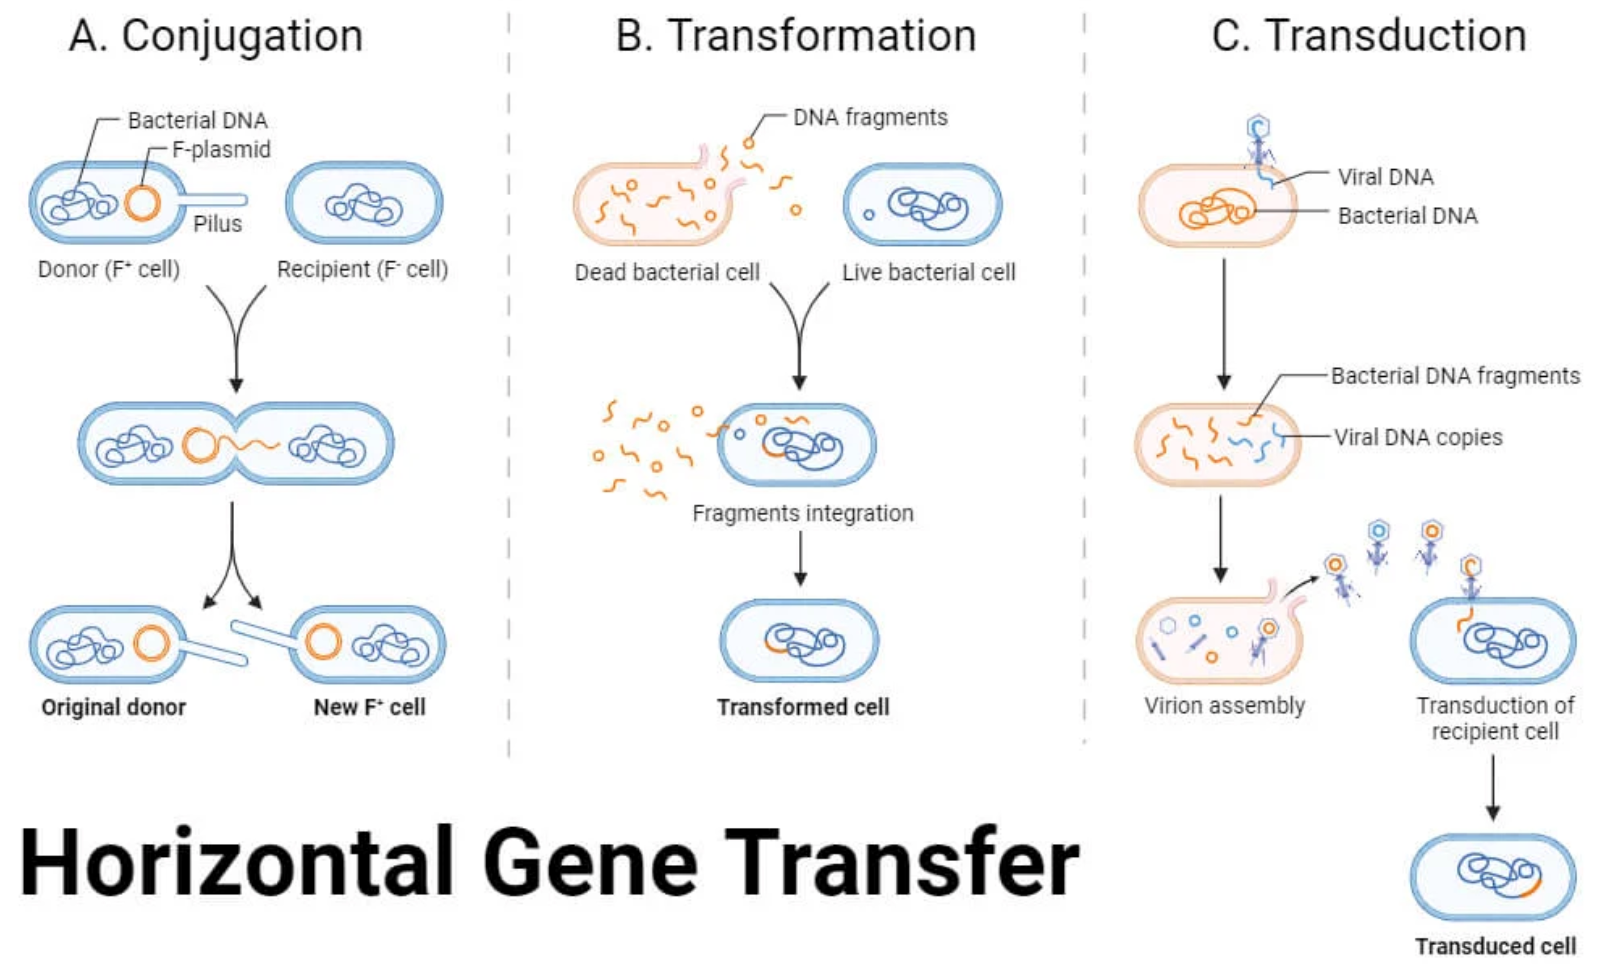
\includegraphics[width=0.7\linewidth]{Figures/horizontal_gene_transfer.png}
    \caption{The three main ways that a (dead) bacterium can transfer DNA over to another bacterium \cite{tamangHorizontalGeneTransfer2023}.}
    \label{fig:horizontal_gene_transfer}
\end{figure}

\subsection{Phage Inactivation and Decoys}
Bacteria can further protect themselves by producing decoys that the phage will attach to instead of themselves, inactivating the phage. 
Freshly lysed bacteria can still contain biomarkers that phages use to detect the bacteria, but upon injection, nothing happens as the cell doesn't function anymore. 
Bacteria can also produce proteolytic enzymes that will damage the proteins found in a phage \cite{tanQuorumSensingDetermines2015}. 
Some bacteria can produce outer membrane vesicles that phages can absorb to, and later detach the vesicle with the phage \cite{rabinovitchBacterialDebrisEcological2003}. 
The vesicle will proceed to float away with the phage attached/injected inside, posing no risk to the source bacteria or to other bacteria. 
It is suspected that the impact of these vesicles acting as a sink is minor \cite{bullPhageBacterialDynamicsSpatial2018}, but helpful nonetheless. 

\subsection{CRISPR-Cas Methods}
CRISPR is a gene editing tool that cells can use to cut out specified/unwanted parts of a DNA strand. 
Researchers are commonly using CRISPR to genetically engineer plants and animals to have specific features. 
Strands of DNA can be selectively added or removed from a DNA strand to achieve a better, more desired DNA strand. 
Specialized defenses in the bacteria can detect unwanted strands and remove the strand, acting as a line of defense against phages. 

\subsection{Phenotype Resistance}

\subsection{Spatial Refuge/Biofilms} 
Usually bacteria and phages coexist in well mixed environments such as the ocean, however some environments offer natural structure for bacteria to hide in. 
These structures can range from physical structure, like reeds in a lake, where the water is stagnant and harder for the phages to diffuse through, to biochemical structures like biofilms, where phages can't diffuse through the biofilm. \newline
Circular bacterial colonies on an agar plate protect the inner bacteria from external phage infections \cite{eriksenGrowingMicrocolonyCan2018}. 
Phages can not swim and do not contain any parts to move. 
They rather rely on passive forms of movement, such as diffusion through the environment or by mixing from environmental factors, such as changes in pressure or heat gradients \cite{lohrmannInfluenceBacterialSwimming2024}. 
Phages rely on Brownian motion, the seemingly random movement of small particles throughout a medium due to other microscopic particles interacting and bouncing off of one another \cite{moineauBacteriophage2013}. 
Unlike phages, bacteria have the ability to actively move through the environment, and can use this to their advantage by swimming away. 
Bacteria and other microbial communities create biofilms, a layer of mucus containing various microbes. 
The thick mucus, microbes, and other spatial effects help protect the bacteria in the biofilm from external phages by making it hard for the phages to penetrate and diffuse through the mucus \cite{abedonPhageDelayEnhancing2017}. 

\subsection{Phage Counter Defense Against Bacteria}
With some of the defenses that bacteria have developed, phages are always mutating to counter their defenses. 
If phages don't adapt to the ever-changing bacterial defenses, the phages will experience an extinction event due to their inability to infect and grow their population count. 
It essentially becomes a race to the bottom, seeing who can out-adapt the other. 
However, if the phages out-adapt the bacteria too much, the bacteria die out, then eventually the phages die out due to not having any bacteria left to infect. 
This can be avoided if the phages can adapt to target a second strain of bacteria, but this is unlikely. 
On the other hand, if bacteria out-adapt the phages, that is no problem for the bacteria because they don't need the phages to survive, and can keep on growing, limited only by the available space and resources. 

This is a problem intrinsic to predator-prey systems, namely that the predators are dependent on the prey. 
Once the prey disappear, the predators also disappear. 
If the prey population goes down, and as a result the predator population goes down and extincts itself, the prey can come back without the threat of predators. 

Phages face this exact same problem: the complete removal of either the bacteria or phages will lead to the removal of the phages from the system unless reintroduced. 

\subsection{Genetic mutations}

\subsection{Viral recombination}
https://www.sciencedirect.com/science/article/pii/S1931312821004170
https://pmc.ncbi.nlm.nih.gov/articles/PMC3185693/
Multiple phages can infect a cell and replicate itself using the cells internal replication process. 
Each phage has its own building blocks. 
Phage 1 could have long legs, a long neck, and a small head, while phage 2 can have long legs, a long neck, and a medium-sized head. 
When the phages are building copies of themselves, they could accidentally use the body parts of other phages. 
The primary method for proteins to bond with other proteins and molecules is via hydrogen bonds. 
These attractive forces hold proteins and other molecules in defined positions, and a change in molecule shape will change the bonds, which will force the other molecule to undergo changes in shape. 
If the proteins that build the subparts of each phage have similar chemical properties, they can be swapped between phages. 
This allows for biological diversity to spread throughout a phage population. 
Each phage body part can have unique characteristics such as better attachment rate, larger DNA storage capsule, or better probability of injection. 

Coexistence between phages and bacteria via genetic co-evolution seems unlikely due to trade-offs imposed by the new mutations \cite{bullOptimalityModelsPhage2006}. 


\section{Phage Defense Against Phages}
Some phages can employ defenses against other phages from infecting the bacterial cell. 
This is called superinfection exclusion (SIE), where a phage that has integrated with the bacterial DNA, called a prophage, prevents a secondary infection from a similar or closely related phage \cite{patelAntiphageDefenceInhibition2024}. 
There are various methods of preventing further infections. 
The phage can alter the surface receptors of the bacteria, making it harder for other phages to detect the bacteria, reducing the chance of attachment and injection by other phages \cite{bucherPhageMachineSIEence2024}. 
Other phages like the T4 phage can use proteins like the Spackle protein. 
The protein inhibits the lysozome activity used in the process of DNA injection by other phages \cite{bucherPhageMachineSIEence2024, kanamaruStructureFunctionT42020}. 
Finally, prophages can encode proteins that will interfere with the replication process of other phages. 
For example, the SieA protein encoded by phage P22 blocks infection from other phages \cite{leavittBacteriophageP22SieAmediated2024}. 

\subsection{Implications of Phage Against Phage Defense}
SIE can affect the speed and development of phage and bacterial populations. A phage restricting other phages from infecting the bacteria creates a competitive environment and can outcompete and dominate the other population. 
This is commonly seen in wildlife populations, where invading species can out compete other species by eating more food/other species faster, breeding at a faster rate than other species, and having no natural predators. 

\subsection{Software Mathematically Modelling Phages, Bacteria, and Resources}
Some software currently exists with the intended goal of modelling phage-bacteria-resource dynamics. 
Cocktail is a simple but yet complex software that models phages in a chemostat system \cite{nilssonCocktailComputerProgram2022}. 
Simple as it has a defined set of parameters, and only considers one resource, one bacteria, and 2 phages, but complex due to the ability for the bacteria to gain phage resistance. 

PhageDyn \cite{krysiak-baltynSimulationPhageDynamics2017} is a Java applet that interacts with existing files in GPS-X \cite{AdvancedWastewaterModelling} to incorporate phage dynamics into models of wastewater treatment plants. 

\subsubsection{Cocktail}
The Cocktail software was developed by Anders S. Nilsson to model phage infection kinetics in a chemostat. 
The model assumes there is one bacteria strain that can be infected by phage A and phage B, and by both phages at the same time, phage AB. 
The bacteria can grow resistance to phage A, phage B, and phage AB independent of one another. 
The model contains inputs controlling bacterial growth rates, decay rate, resistance mutation rate against phage A, phage B, and against phage AB. 
The software as settings for controlling the resource concentration, available supply, and flow rate of the resource. 
Finally, the user can control the parameter values for phage A and B, such as the adsorption rate, patent period, and burst size. 
There is an option to periodically add more phages. 
Finally there are some settings to control the model settings, such as if the model is deterministic or stochastic, and the step size \cite{nilssonCocktailComputerProgram2022}. 
After choosing the parameter values, an output is created, with four sample plots shown in \Cref{fig:cocktail_software_output}
\begin{figure}
    \centering
    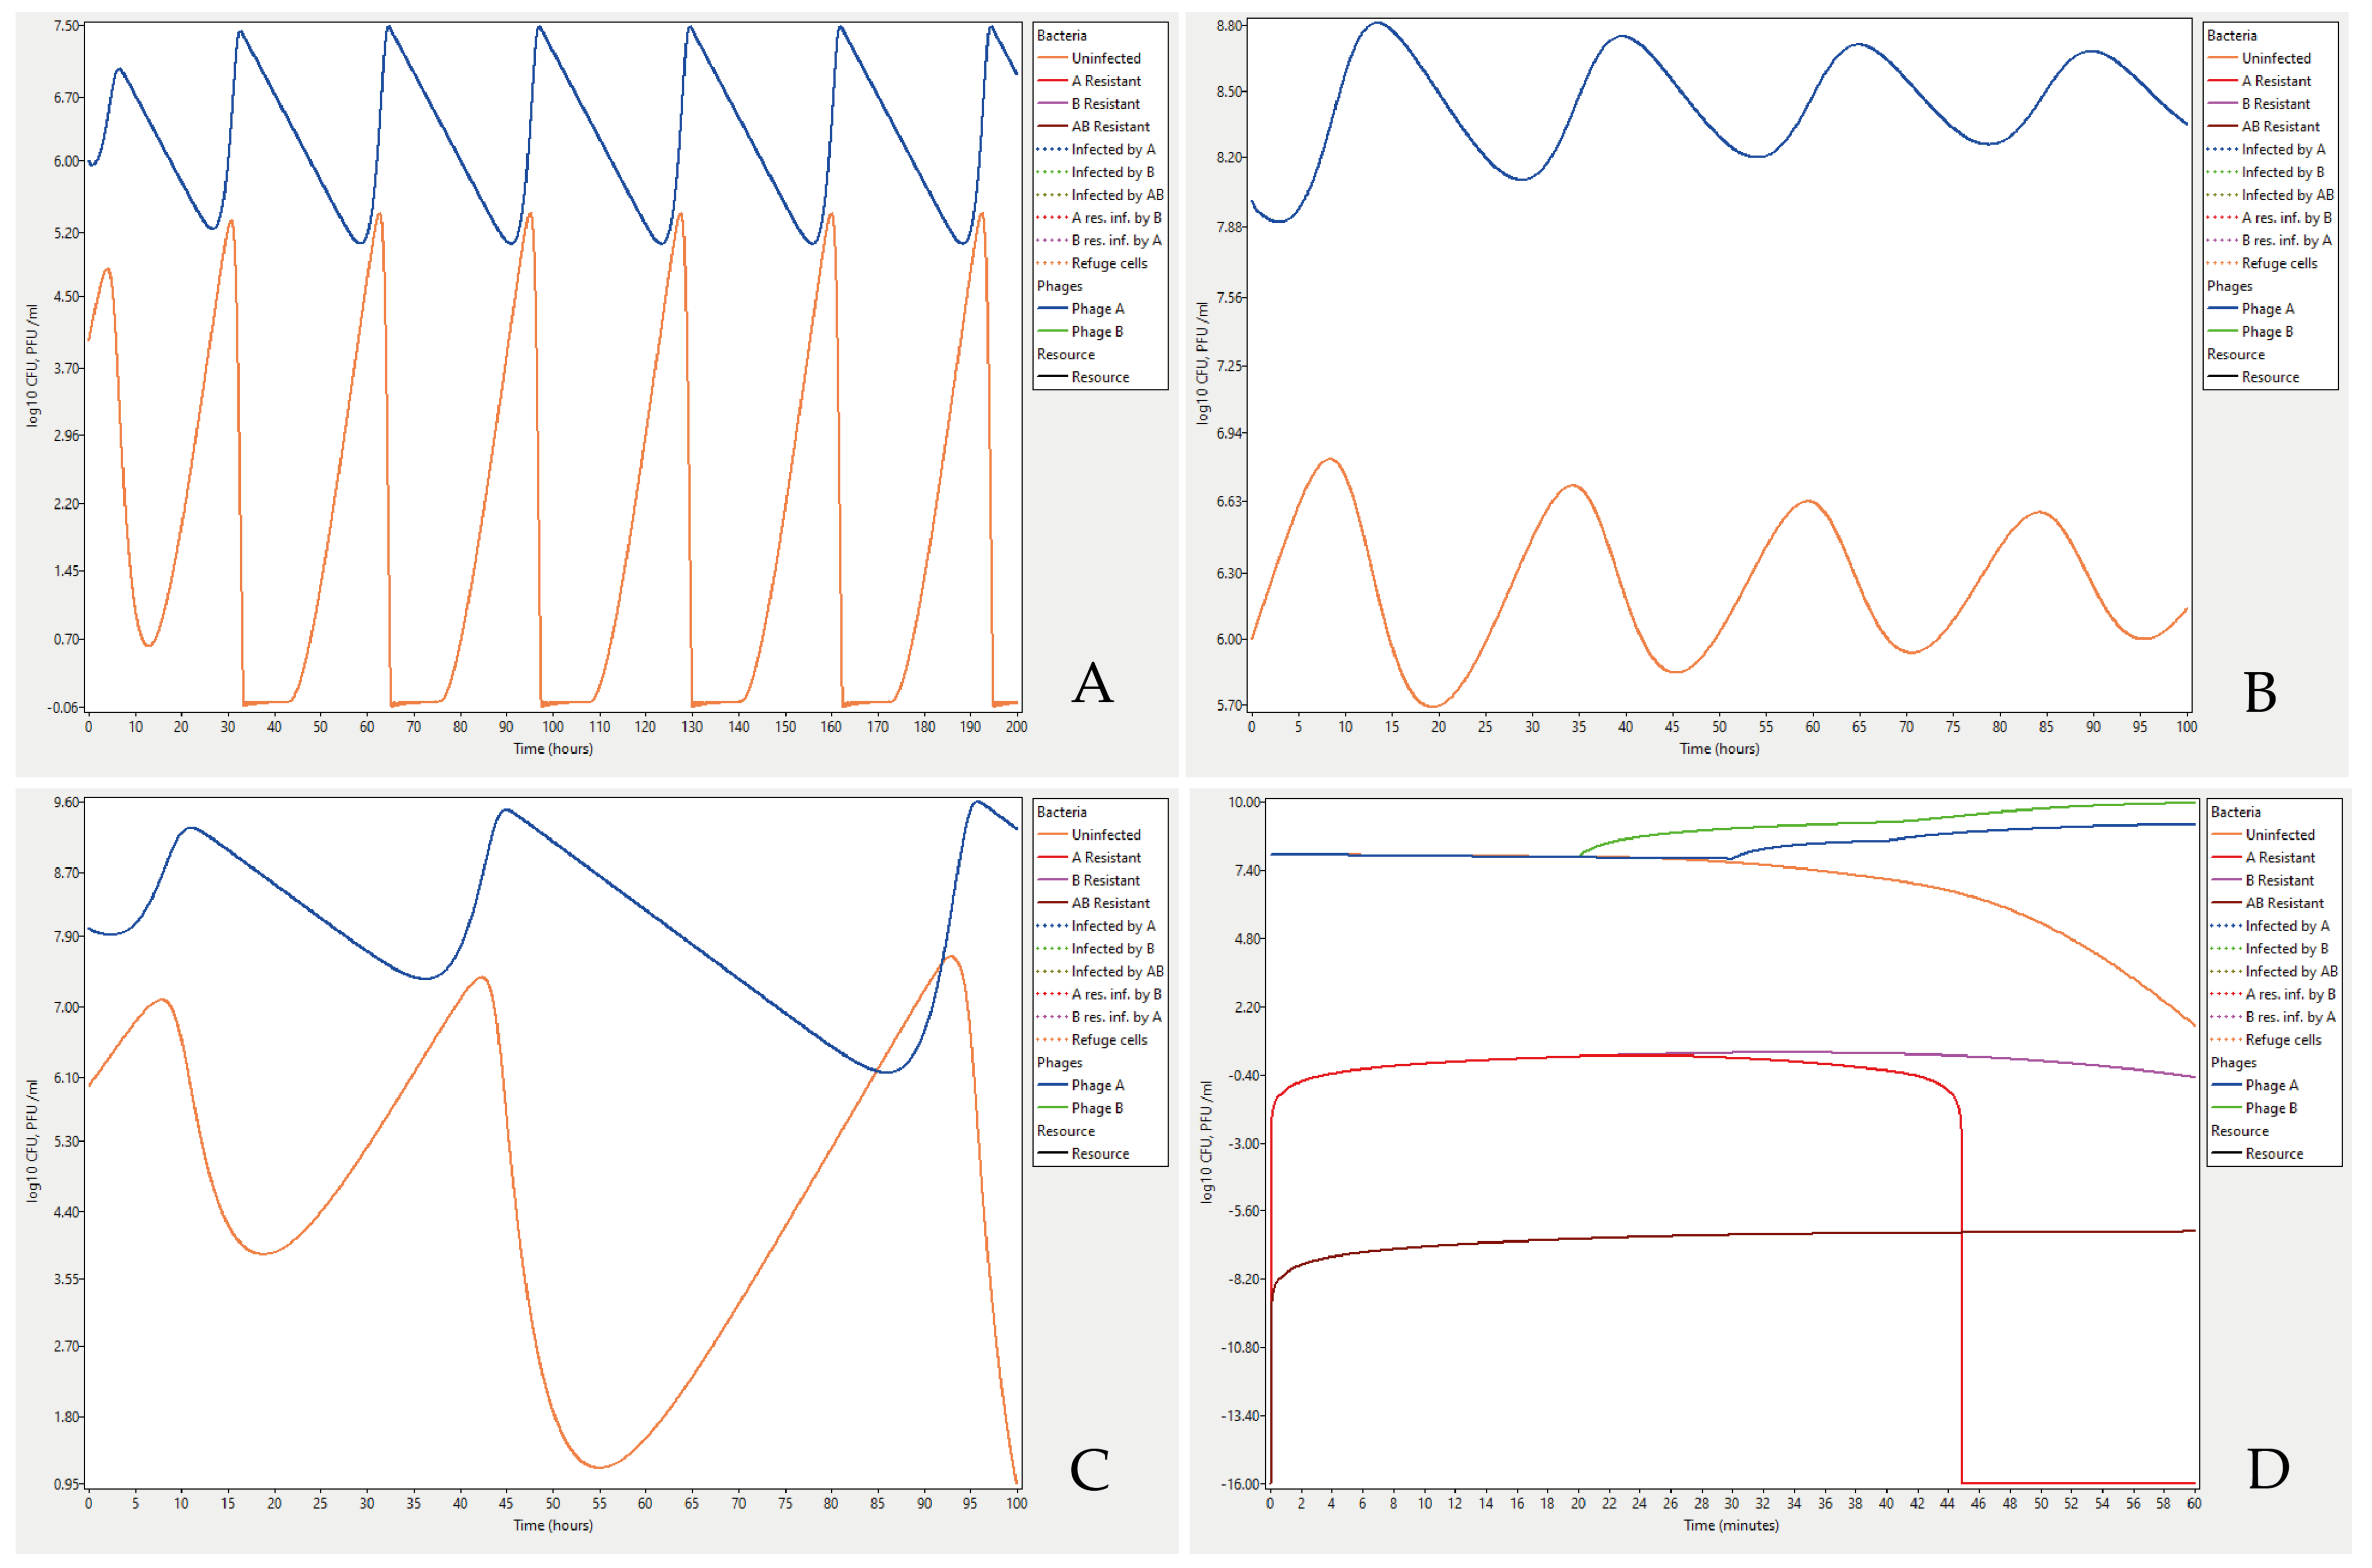
\includegraphics[width=0.7\linewidth]{Plots/Sourced/cocktail_plot.png}
    \caption{
        Example output from Cocktail. \newline
        \raggedright
        Figure A) \textit{E. coli} infected with phage T4 in a chemostat exhibiting an oscillating growth behavior, following the model of \citet{bohannanEffectResourceEnrichment1997}. \\
        Figure B) Oscillations of bacteria and phages can exist at higher titers, dependent on low resource concentration, following the model of \citet{lenskiDynamicsInteractionsBacteria1988}. \\
        Figure C) As the concentration of resources change, this results in increasing oscillations, but not going extinct. \\
        Figure D) A system modelling the interactions with phage A and B. \\
        See \citet{nilssonCocktailComputerProgram2022} for more information on parameter values, sources, and supplementary resources. 
    }
    \label{fig:cocktail_software_output}
\end{figure}

\subsubsection{PhageDyn}
PhageDyn is an add-on for the commercial software GPS-X, an advanced wastewater and industrial wastewater treatment plants modelling simulation software created by Hydromantis Inc. 
The aim of the software is to model phage dynamics in multi-reactor models. 
Previous attempts at modelling phage dynamics are not applicable to a complex multi-reactor wastewater treatment plant model. 
PhageDyn models the behavior of phages in multiple interconnected reactors with the aim of reducing foaming in wastewater treatment plants caused by bacteria \cite{heardEffectFilamentousBacteria2008}. \Cref{fig:PhageDyn_software_output} shows the output 
\begin{figure}
    \centering
    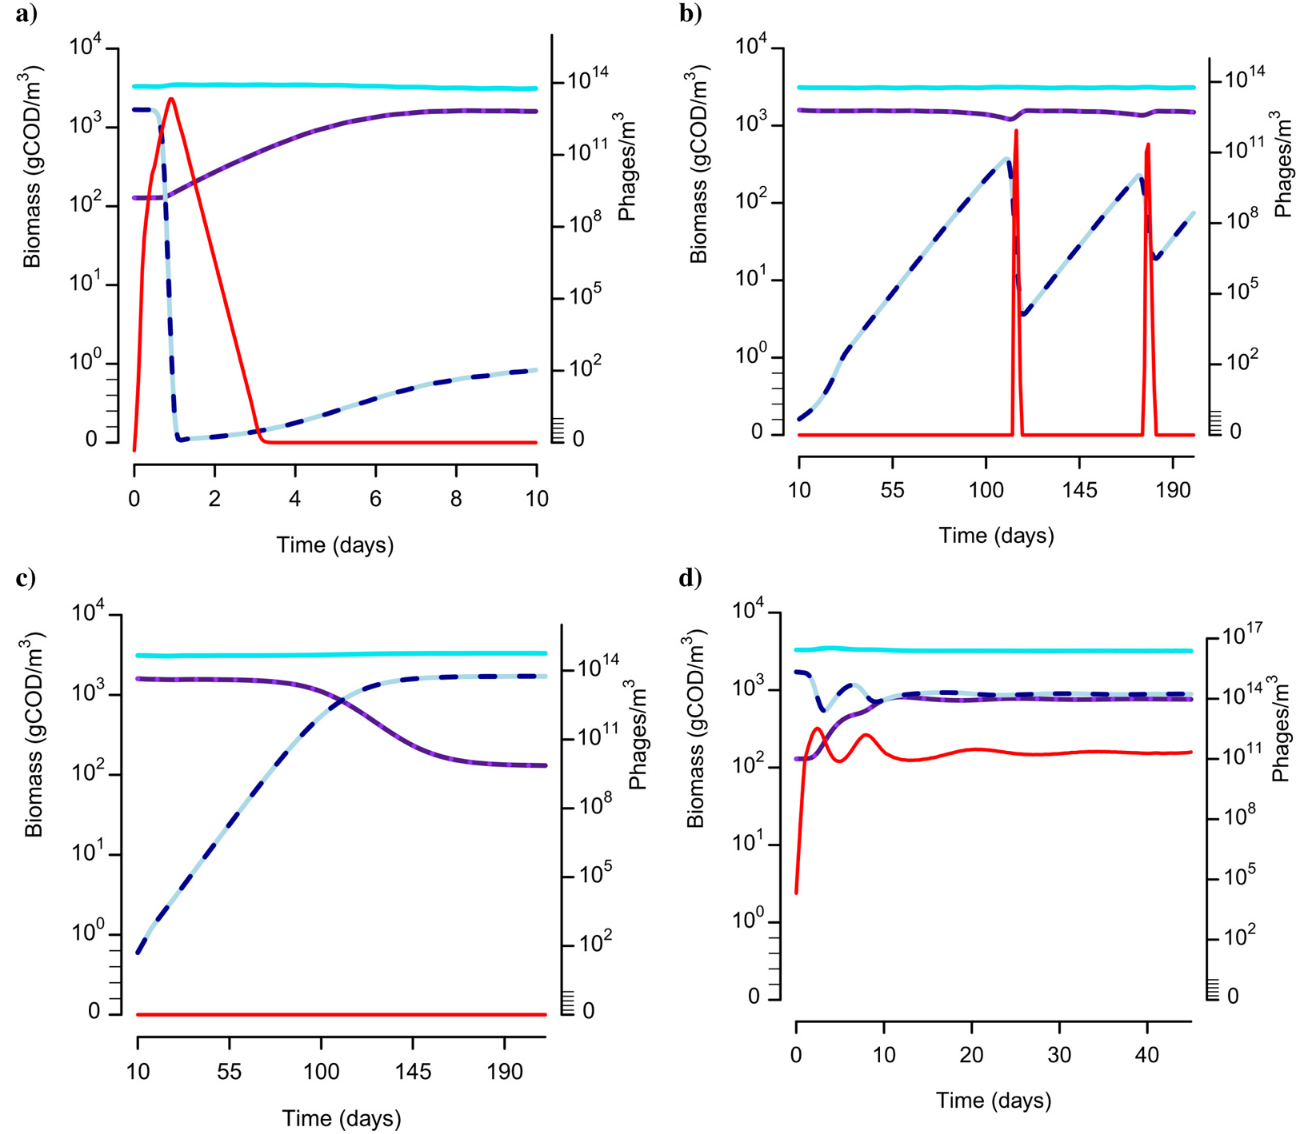
\includegraphics[width=0.7\linewidth]{Plots/Sourced/phagedyn_plot.png}
    \caption{
        Example output from PhageDyn, showing concentration of heterotrophic biomass in an aerobic plug flow across four situations.
        \textcolor[HTML]{551A8C}{\textbf{Purple}} is heterotrophic biomass, 
        \textcolor[HTML]{4580B4}{\textbf{Blue}} is foaming biomass, 
        \textcolor[HTML]{FF0000}{\textbf{Red}} is phages, 
        \textcolor[HTML]{01E6EE}{\textbf{Light Blue}} is total suspended solids. \\
        \raggedright
        Figure A) Biomass concentration immediately post phage dosing. \\
        Figure B) Biomass concentration with low phage concentration and maintain low concentration post spike in population count. \\
        Figure C) Biomass concentration when phages are extinct. \\
        Figure D) Biomass concentration with a less virulent and low adsorption rate phage, co-existence with biomass reached. \\
        A change in phage concentration shows a decrease in heterotrophic and foaming biomass. \cite{krysiak-baltynSimulationPhageDynamics2017}
    }
    \label{fig:PhageDyn_software_output}
\end{figure}
